% Created 2024-05-12 Sun 23:07
% Intended LaTeX compiler: pdflatex
\documentclass[12pt]{article}

%%%% settings when exporting code %%%% 

\usepackage{listings}
\lstdefinestyle{code-small}{
backgroundcolor=\color{white}, % background color for the code block
basicstyle=\ttfamily\small, % font used to display the code
commentstyle=\color[rgb]{0.5,0,0.5}, % color used to display comments in the code
keywordstyle=\color{black}, % color used to highlight certain words in the code
numberstyle=\ttfamily\tiny\color{gray}, % color used to display the line numbers
rulecolor=\color{black}, % color of the frame
stringstyle=\color[rgb]{0,.5,0},  % color used to display strings in the code
breakatwhitespace=false, % sets if automatic breaks should only happen at whitespace
breaklines=true, % sets automatic line breaking
columns=fullflexible,
frame=single, % adds a frame around the code (non,leftline,topline,bottomline,lines,single,shadowbox)
keepspaces=true, % % keeps spaces in text, useful for keeping indentation of code
literate={~}{$\sim$}{1}, % symbol properly display via latex
numbers=none, % where to put the line-numbers; possible values are (none, left, right)
numbersep=10pt, % how far the line-numbers are from the code
showspaces=false,
showstringspaces=false,
stepnumber=1, % the step between two line-numbers. If it's 1, each line will be numbered
tabsize=1,
xleftmargin=0cm,
emph={anova,apply,class,coef,colnames,colNames,colSums,dim,dcast,for,ggplot,head,if,ifelse,is.na,lapply,list.files,library,logLik,melt,plot,require,rowSums,sapply,setcolorder,setkey,str,summary,tapply},
aboveskip = \medskipamount, % define the space above displayed listings.
belowskip = \medskipamount, % define the space above displayed listings.
lineskip = 0pt} % specifies additional space between lines in listings
\lstset{style=code-small}
%%%% packages %%%%%

\usepackage[utf8]{inputenc}
\usepackage[T1]{fontenc}
\usepackage{lmodern}
\usepackage{textcomp}
\usepackage{color}
\usepackage{graphicx}
\usepackage{grffile}
\usepackage{wrapfig}
\usepackage{rotating}
\usepackage{longtable}
\usepackage{multirow}
\usepackage{multicol}
\usepackage{changes}
\usepackage{pdflscape}
\usepackage{geometry}
\usepackage[normalem]{ulem}
\usepackage{amssymb}
\usepackage{amsmath}
\usepackage{amsfonts}
\usepackage{dsfont}
\usepackage{array}
\usepackage{ifthen}
\usepackage{hyperref}
\usepackage{natbib}
\RequirePackage{setspace} % to modify the space between lines - incompatible with footnote in beamer
\renewcommand{\baselinestretch}{1.1}
\geometry{a4paper, left=10mm, right=10mm, top=10mm}
\usepackage{titlesec}
\usepackage{etoolbox}

\makeatletter
\patchcmd{\ttlh@hang}{\parindent\z@}{\parindent\z@\leavevmode}{}{}
\patchcmd{\ttlh@hang}{\noindent}{}{}{}
\makeatother
\RequirePackage{colortbl} % arrayrulecolor to mix colors
\definecolor{myorange}{rgb}{1,0.2,0}
\definecolor{mypurple}{rgb}{0.7,0,8}
\definecolor{mycyan}{rgb}{0,0.6,0.6}
\newcommand{\lightblue}{blue!50!white}
\newcommand{\darkblue}{blue!80!black}
\newcommand{\darkgreen}{green!50!black}
\newcommand{\darkred}{red!50!black}
\definecolor{gray}{gray}{0.5}
\hypersetup{
citecolor=[rgb]{0,0.5,0},
urlcolor=[rgb]{0,0,0.5},
linkcolor=[rgb]{0,0,0.5},
}
\newenvironment{note}{\small \color{gray}\fontfamily{lmtt}\selectfont}{\par}
\newenvironment{activity}{\color{orange}\fontfamily{qzc}\selectfont}{\par}
\RequirePackage{pifont}
\RequirePackage{relsize}
\newcommand{\Cross}{{\raisebox{-0.5ex}%
{\relsize{1.5}\ding{56}}}\hspace{1pt} }
\newcommand{\Valid}{{\raisebox{-0.5ex}%
{\relsize{1.5}\ding{52}}}\hspace{1pt} }
\newcommand{\CrossR}{ \textcolor{red}{\Cross} }
\newcommand{\ValidV}{ \textcolor{green}{\Valid} }
\usepackage{stackengine}
\usepackage{scalerel}
\newcommand\Warning[1][3ex]{%
\renewcommand\stacktype{L}%
\scaleto{\stackon[1.3pt]{\color{red}$\triangle$}{\tiny\bfseries !}}{#1}%
\xspace
}
\RequirePackage{fancyvrb}
\DefineVerbatimEnvironment{verbatim}{Verbatim}{fontsize=\small,formatcom = {\color[rgb]{0.5,0,0}}}
\definecolor{grayR}{HTML}{8A8990}
\definecolor{grayL}{HTML}{C4C7C9}
\definecolor{blueM}{HTML}{1F63B5}
\newcommand{\Rlogo}[1][0.07]{
\begin{tikzpicture}[scale=#1]
\shade [right color=grayR,left color=grayL,shading angle=60]
(-3.55,0.3) .. controls (-3.55,1.75)
and (-1.9,2.7) .. (0,2.7) .. controls (2.05,2.7)
and (3.5,1.6) .. (3.5,0.3) .. controls (3.5,-1.2)
and (1.55,-2) .. (0,-2) .. controls (-2.3,-2)
and (-3.55,-0.75) .. cycle;

\fill[white]
(-2.15,0.2) .. controls (-2.15,1.2)
and (-0.7,1.8) .. (0.5,1.8) .. controls (2.2,1.8)
and (3.1,1.2) .. (3.1,0.2) .. controls (3.1,-0.75)
and (2.4,-1.45) .. (0.5,-1.45) .. controls (-1.1,-1.45)
and (-2.15,-0.7) .. cycle;

\fill[blueM]
(1.75,1.25) -- (-0.65,1.25) -- (-0.65,-2.75) -- (0.55,-2.75) -- (0.55,-1.15) --
(0.95,-1.15)  .. controls (1.15,-1.15)
and (1.5,-1.9) .. (1.9,-2.75) -- (3.25,-2.75)  .. controls (2.2,-1)
and (2.5,-1.2) .. (1.8,-0.95) .. controls (2.6,-0.9)
and (2.85,-0.35) .. (2.85,0.2) .. controls (2.85,0.7)
and (2.5,1.2) .. cycle;

\fill[white]  (1.4,0.4) -- (0.55,0.4) -- (0.55,-0.3) -- (1.4,-0.3).. controls (1.75,-0.3)
and (1.75,0.4) .. cycle;

\end{tikzpicture}
}
\RequirePackage{epstopdf} % to be able to convert .eps to .pdf image files
\RequirePackage{capt-of} %
\RequirePackage{caption} % newlines in graphics
\RequirePackage{tikz-cd} % graph
\RequirePackage{booktabs} % for nice lines in table (e.g. toprule, bottomrule, midrule, cmidrule)
\RequirePackage{amsmath}
\RequirePackage{algorithm}
\RequirePackage[noend]{algpseudocode}
\RequirePackage{dsfont}
\RequirePackage{amsmath,stmaryrd,graphicx}
\RequirePackage{prodint} % product integral symbol (\PRODI)
\usepackage{ifthen}
\usepackage{xifthen}
\usepackage{xargs}
\usepackage{xspace}
\newcommand\defOperator[7]{%
\ifthenelse{\isempty{#2}}{
\ifthenelse{\isempty{#1}}{#7{#3}#4}{#7{#3}#4 \left#5 #1 \right#6}
}{
\ifthenelse{\isempty{#1}}{#7{#3}#4_{#2}}{#7{#3}#4_{#1}\left#5 #2 \right#6}
}
}
\newcommand\defUOperator[5]{%
\ifthenelse{\isempty{#1}}{
#5\left#3 #2 \right#4
}{
\ifthenelse{\isempty{#2}}{\underset{#1}{\operatornamewithlimits{#5}}}{
\underset{#1}{\operatornamewithlimits{#5}}\left#3 #2 \right#4}
}
}
\newcommand{\defBoldVar}[2]{
\ifthenelse{\equal{#2}{T}}{\boldsymbol{#1}}{\mathbf{#1}}
}
\newcommandx\Esp[2][1=,2=]{\defOperator{#1}{#2}{E}{}{\lbrack}{\rbrack}{\mathbb}}
\newcommandx\Prob[2][1=,2=]{\defOperator{#1}{#2}{P}{}{\lbrack}{\rbrack}{\mathbb}}
\newcommandx\Qrob[2][1=,2=]{\defOperator{#1}{#2}{Q}{}{\lbrack}{\rbrack}{\mathbb}}
\newcommandx\Var[2][1=,2=]{\defOperator{#1}{#2}{V}{ar}{\lbrack}{\rbrack}{\mathbb}}
\newcommandx\Cov[2][1=,2=]{\defOperator{#1}{#2}{C}{ov}{\lbrack}{\rbrack}{\mathbb}}
\newcommandx\Binom[2][1=,2=]{\defOperator{#1}{#2}{B}{}{(}{)}{\mathcal}}
\newcommandx\Gaus[2][1=,2=]{\defOperator{#1}{#2}{N}{}{(}{)}{\mathcal}}
\newcommandx\Wishart[2][1=,2=]{\defOperator{#1}{#2}{W}{ishart}{(}{)}{\mathcal}}
\newcommandx\Likelihood[2][1=,2=]{\defOperator{#1}{#2}{L}{}{(}{)}{\mathcal}}
\newcommandx\logLikelihood[2][1=,2=]{\defOperator{#1}{#2}{\ell}{}{(}{)}{}}
\newcommandx\Information[2][1=,2=]{\defOperator{#1}{#2}{I}{}{(}{)}{\mathcal}}
\newcommandx\Hessian[2][1=,2=]{\defOperator{#1}{#2}{H}{}{(}{)}{\mathcal}}
\newcommandx\Score[2][1=,2=]{\defOperator{#1}{#2}{S}{}{(}{)}{\mathcal}}
\newcommandx\Vois[2][1=,2=]{\defOperator{#1}{#2}{V}{}{(}{)}{\mathcal}}
\newcommandx\IF[2][1=,2=]{\defOperator{#1}{#2}{IF}{}{(}{)}{\mathcal}}
\newcommandx\Ind[1][1=]{\defOperator{}{#1}{1}{}{(}{)}{\mathds}}
\newcommandx\Max[2][1=,2=]{\defUOperator{#1}{#2}{(}{)}{min}}
\newcommandx\Min[2][1=,2=]{\defUOperator{#1}{#2}{(}{)}{max}}
\newcommandx\argMax[2][1=,2=]{\defUOperator{#1}{#2}{(}{)}{argmax}}
\newcommandx\argMin[2][1=,2=]{\defUOperator{#1}{#2}{(}{)}{argmin}}
\newcommandx\cvD[2][1=D,2=n \rightarrow \infty]{\xrightarrow[#2]{#1}}
\newcommandx\Hypothesis[2][1=,2=]{
\ifthenelse{\isempty{#1}}{
\mathcal{H}
}{
\ifthenelse{\isempty{#2}}{
\mathcal{H}_{#1}
}{
\mathcal{H}^{(#2)}_{#1}
}
}
}
\newcommandx\dpartial[4][1=,2=,3=,4=\partial]{
\ifthenelse{\isempty{#3}}{
\frac{#4 #1}{#4 #2}
}{
\left.\frac{#4 #1}{#4 #2}\right\rvert_{#3}
}
}
\newcommandx\dTpartial[3][1=,2=,3=]{\dpartial[#1][#2][#3][d]}
\newcommandx\ddpartial[3][1=,2=,3=]{
\ifthenelse{\isempty{#3}}{
\frac{\partial^{2} #1}{\partial #2^2}
}{
\frac{\partial^2 #1}{\partial #2\partial #3}
}
}
\newcommand\Real{\mathbb{R}}
\newcommand\Rational{\mathbb{Q}}
\newcommand\Natural{\mathbb{N}}
\newcommand\trans[1]{{#1}^\intercal}%\newcommand\trans[1]{{\vphantom{#1}}^\top{#1}}
\newcommand{\independent}{\mathrel{\text{\scalebox{1.5}{$\perp\mkern-10mu\perp$}}}}
\newcommand\half{\frac{1}{2}}
\newcommand\normMax[1]{\left|\left|#1\right|\right|_{max}}
\newcommand\normTwo[1]{\left|\left|#1\right|\right|_{2}}
\newcommand\Veta{\boldsymbol{\eta}}
\newcommand{\Model}{\mathcal{M}}
\newcommand{\ModelHat}{\widehat{\mathcal{M}}}
\newcommand{\param}{\Theta}
\newcommand{\paramHat}{\widehat{\param}}
\newcommand{\paramCon}{\widetilde{\param}}
\newcommand{\Vparam}{\boldsymbol{\param}}
\newcommand{\VparamT}{\Vparam_0}
\newcommand{\VparamHat}{\boldsymbol{\paramHat}}
\newcommand{\VparamCon}{\boldsymbol{\paramCon}}
\newcommand{\X}{X}
\newcommand{\x}{x}
\newcommand{\VZ}{\boldsymbol{Z}}
\newcommand{\VX}{\boldsymbol{X}}
\newcommand{\Vx}{\boldsymbol{x}}
\newcommand{\Y}{Y}
\newcommand{\y}{y}
\newcommand{\VY}{\boldsymbol{Y}}
\newcommand{\Vy}{\boldsymbol{y}}
\newcommand{\Vvarepsilon}{\boldsymbol{\varepsilon}}
\author{Brice Ozenne}
\date{\today}
\title{Partial residuals with the package LMMstar}
\hypersetup{
 colorlinks=true,
 pdfauthor={Brice Ozenne},
 pdftitle={Partial residuals with the package LMMstar},
 pdfkeywords={},
 pdfsubject={},
 pdfcreator={Emacs 27.1 (Org mode 9.4.6)},
 pdflang={English}
 }
\begin{document}

\maketitle
This vignette details how partial residuals can be used to illustrate
model fit in a linear regression and a linear mixed model when using
the package LMMstar. We thus start by loading the necessary packages:
\lstset{language=r,label= ,caption= ,captionpos=b,numbers=none}
\begin{lstlisting}
library(LMMstar)
library(ggplot2)
\end{lstlisting}


\section{Univariate linear regression}
\label{sec:org82717b8}

To illustrate the use of partial residuals we will use the \texttt{state.x77}
dataset:
\lstset{language=r,label= ,caption= ,captionpos=b,numbers=none}
\begin{lstlisting}
df1 <- data.frame(lifeExp = state.x77[,4],
                  illiteracy = state.x77[,3],
                  income = state.x77[,2]/1000,
                  murder = state.x77[,5],
                  edu = cut(state.x77[,6],c(0,50,60,100)))
head(df1,4)
\end{lstlisting}

\begin{verbatim}
         lifeExp illiteracy income murder      edu
Alabama    69.05        2.1  3.624   15.1   (0,50]
Alaska     69.31        1.5  6.315   11.3 (60,100]
Arizona    70.55        1.8  4.530    7.8  (50,60]
Arkansas   70.66        1.9  3.378   10.1   (0,50]
\end{verbatim}


 which contains information about life expectancy (\texttt{lifeExp}), income
(\texttt{income}), illeteracy (\texttt{illiteracy}), murder rate (\texttt{murder}), and the
percentage of high-school graduates (as categorical variable) in
various states in the USA. For later use we display a few descriptive
for each covariate value:
\lstset{language=r,label= ,caption= ,captionpos=b,numbers=none}
\begin{lstlisting}
summarize(lifeExp + illiteracy + income + murder + edu ~ 1, data = df1,
          columns = c("observed","missing","mean","min","max","sd"))
\end{lstlisting}

\begin{verbatim}
       outcome observed missing    mean    min    max      sd
1      lifeExp       50       0 70.8786 67.960 73.600 1.34239
2   illiteracy       50       0  1.1700  0.500  2.800 0.60953
3       income       50       0  4.4358  3.098  6.315 0.61447
4       murder       50       0  7.3780  1.400 15.100 3.69154
5  edu:(50,60]       50       0  0.5600  0.000  1.000 0.50143
6 edu:(60,100]       50       0  0.1600  0.000  1.000 0.37033
\end{verbatim}


and check there are no missing values. Here for the categorical
covariates the mean indicates the relative frequency of occurrence
(56\% and 16\%) and other columns like \texttt{sd} should be ignored.

\subsection{No interaction}
\label{sec:orgb0c8955}

Suppose we are interested in relating life expectancy (\(Y\)) to
income (\(X\)). We cannot directly illustrate this relationship, as it
could be confounded by other variables such as illiteracy (\(Z_1\)),
murder rate (\(Z_2\)). and education (\(Z_3\)). We will therefore use
a linear model to control for those variables (\(\VZ=(Z_1,Z_2,Z_3)\))
where, for simplicity, we assume a linear effect for all variables:
\begin{align*}
Y = \alpha + \beta X + \gamma_1 Z_1 + \gamma_2 Z_2 + \gamma_2 Z_3 + \varepsilon
\end{align*}
\lstset{language=r,label= ,caption= ,captionpos=b,numbers=none}
\begin{lstlisting}
e.lm <- lmm(lifeExp ~ income + illiteracy + murder + edu, data = df1)
model.tables(e.lm)
\end{lstlisting}

\begin{verbatim}
            estimate       se     df    lower    upper    p.value
(Intercept) 71.57828 1.138488 44.009 69.28382 73.87274 0.0000e+00
income       0.19270 0.252649 44.009 -0.31648  0.70188 4.4971e-01
illiteracy   0.17590 0.320967 44.009 -0.47096  0.82276 5.8644e-01
murder      -0.27822 0.047855 44.009 -0.37467 -0.18178 6.3280e-07
edu(50,60]   0.30141 0.414015 44.009 -0.53298  1.13580 4.7046e-01
edu(60,100]  0.77306 0.513118 44.009 -0.26105  1.80718 1.3906e-01
\end{verbatim}


Note that the estimates are nearly identical to the ones of the \texttt{lm}
function:
\lstset{language=r,label= ,caption= ,captionpos=b,numbers=none}
\begin{lstlisting}
coef(e.lm) - coef(lm(lifeExp ~ income + illiteracy + murder + edu, data = df1))
\end{lstlisting}

\begin{verbatim}
(Intercept)      income  illiteracy      murder  edu(50,60] edu(60,100] 
-2.7001e-13  2.0345e-13 -2.9035e-13  6.3283e-15 -4.2277e-13 -5.3091e-13
\end{verbatim}


A graphical display can now be obtained by modifying the original
outcome, life expectancy, had every state had the same illiteracy and
murder rate:
\lstset{language=r,label= ,caption= ,captionpos=b,numbers=none}
\begin{lstlisting}
df1$pres <- residuals(e.lm, type = "partial", variable = c("(Intercept)","income"))
head(df1)
\end{lstlisting}

\begin{verbatim}
           lifeExp illiteracy income murder      edu   pres
Alabama      69.05        2.1  3.624   15.1   (0,50] 72.882
Alaska       69.31        1.5  6.315   11.3 (60,100] 71.417
Arizona      70.55        1.8  4.530    7.8  (50,60] 72.102
Arkansas     70.66        1.9  3.378   10.1   (0,50] 73.136
California   71.71        1.1  5.114   10.3 (60,100] 73.609
Colorado     72.06        0.7  4.884    6.8 (60,100] 73.056
\end{verbatim}


By default, the partial residuals are computed substracting the effect
of the covariates, i.e. had each state got no illiteracy, no murder,
and the lowest education level:
\lstset{language=r,label= ,caption= ,captionpos=b,numbers=none}
\begin{lstlisting}
c(69.05 - 0.17590 * 2.1 - (-0.27822) * 15.1,
  69.31 - 0.17590 * 1.5 - (-0.27822) * 11.3 - 0.77306)
\end{lstlisting}

\begin{verbatim}
[1] 72.882 71.417
\end{verbatim}


The element \texttt{"(Intercept)"} was specified in the \texttt{variable} argument
to avoid to substract the mean value from the outcome and keep a
plausible range of values for the outcome.

\bigskip

One may wish to compute the life expectancy had every state got a
specific illiteracy, murder rate, and education. Say the most common
in the sample: 1.17, 7.378, and (50,60] based on the descriptive
statistics. This can be obtained by specifying these values in the
argument \texttt{at}:
\lstset{language=r,label= ,caption= ,captionpos=b,numbers=none}
\begin{lstlisting}
df1$pres2 <- residuals(e.lm, type = "partial", variable = c("(Intercept)","income"),
                       at = data.frame(illiteracy = 1.17, murder = 7.378, edu = "(50,60]"))
head(df1)
\end{lstlisting}

\begin{verbatim}
           lifeExp illiteracy income murder      edu   pres  pres2
Alabama      69.05        2.1  3.624   15.1   (0,50] 72.882 71.336
Alaska       69.31        1.5  6.315   11.3 (60,100] 71.417 69.871
Arizona      70.55        1.8  4.530    7.8  (50,60] 72.102 70.557
Arkansas     70.66        1.9  3.378   10.1   (0,50] 73.136 71.590
California   71.71        1.1  5.114   10.3 (60,100] 73.609 72.064
Colorado     72.06        0.7  4.884    6.8 (60,100] 73.056 71.510
\end{verbatim}


or doing the calcuation by hand:
\lstset{language=r,label= ,caption= ,captionpos=b,numbers=none}
\begin{lstlisting}
c(69.05 - 0.17590 * (2.1-1.170) - (-0.27822) * (15.1-7.378) + 0.30141,
  69.31 - 0.17590 * (1.5-1.170) - (-0.27822) * (11.3-7.378) + 0.30141 - 0.77306)
\end{lstlisting}

\begin{verbatim}
[1] 71.336 69.871
\end{verbatim}


Note that changing in counterfactual only shifts the partial residuals
by a constant, here:
\lstset{language=r,label= ,caption= ,captionpos=b,numbers=none}
\begin{lstlisting}
unique(df1$pres2 - df1$pres)
\end{lstlisting}

\begin{verbatim}
[1] -1.5455
\end{verbatim}


so does not affect the relation between the counterfactual outcome
(here \texttt{lifeExp}) and the exposure of interest (here \texttt{income}). One can
then get a graphical display either manually using ggplot:
\lstset{language=r,label= ,caption= ,captionpos=b,numbers=none}
\begin{lstlisting}
gg.pres <- ggplot(df1) + geom_point(aes(x=income, y=pres))
gg.pres <- gg.pres + geom_abline(intercept = coef(e.lm)["(Intercept)"],
                                 slope = coef(e.lm)["income"])
gg.pres <- gg.pres + ggtitle("(B) partial residuals")
gg.pres
\end{lstlisting}

or directly via the plot function:
\lstset{language=r,label= ,caption= ,captionpos=b,numbers=none}
\begin{lstlisting}
plot(e.lm, type = "partial", variable = c("(Intercept)","income")) # C
plot(e.lm, type = "partial", variable = c("(Intercept)","income"),
     at = data.frame(illiteracy = 1.17, murder = 7.378, edu = "(50,60]")) # D
\end{lstlisting}

\clearpage

These can be compared to displaying the observed outcome vs. income:
\lstset{language=r,label= ,caption= ,captionpos=b,numbers=none}
\begin{lstlisting}
gg.obs <- ggplot(df1) + geom_point(aes(x=income, y=lifeExp))
gg.obs <- gg.obs + ggtitle("(A) observed")
gg.obs
\end{lstlisting}

where it is apparent that by using the partial residuals, the data has
been normalized and exhibit less variability.
\begin{center}
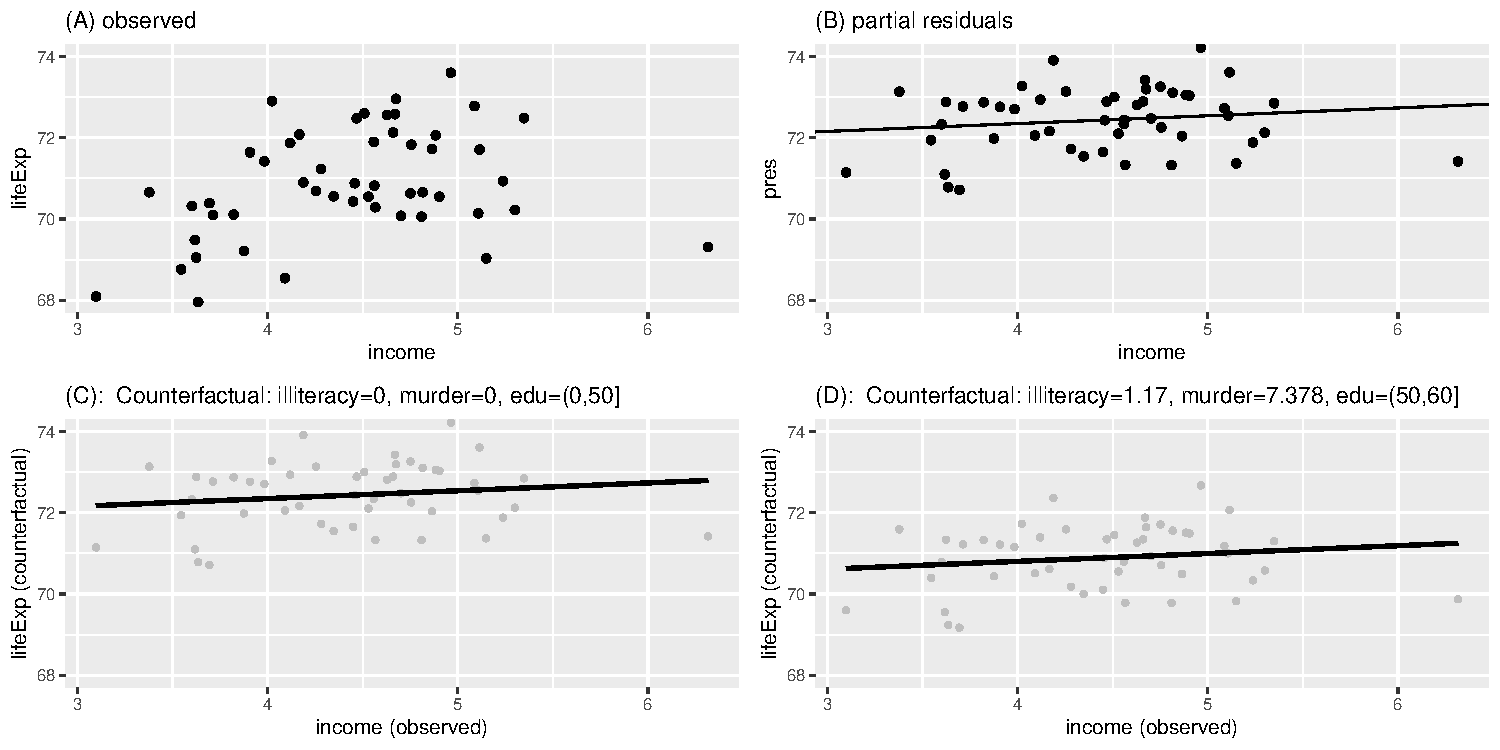
\includegraphics[trim={0 0 0 0},width=1\textwidth]{./figures/gg-lmpres-comparisons.pdf}
\end{center}

The output of the \texttt{plot} method is a list containing an element plot
with the ggplot object and an element data with the dataset. To avoid
actually displaying the graph one can use the method \texttt{autoplot} to
only save the ggplot object:
\lstset{language=r,label= ,caption= ,captionpos=b,numbers=none}
\begin{lstlisting}
ls.plot <- autoplot(e.lm, type = "partial", variable = c("(Intercept)","income"))
lapply(ls.plot, class)
\end{lstlisting}

\begin{verbatim}
$data
[1] "residuals_lmm" "data.frame"   

$plot
[1] "gg"     "ggplot"
\end{verbatim}


One can re-create the plot based on the data argument or modify the
existing plot, e.g. displaying with the y axis between 68 and 74:
\lstset{language=r,label= ,caption= ,captionpos=b,numbers=none}
\begin{lstlisting}
ls.plot$plot  + coord_cartesian(ylim=c(68,74))
\end{lstlisting}

\bigskip

\subsection{What about confidence intervals?}
\label{sec:org344baf0}

A common question is whether one can display confidence intervals for
the regression line. It is possible to add confidence intervals on the
plot either via the argument \texttt{ci.alpha}:
\lstset{language=r,label= ,caption= ,captionpos=b,numbers=none}
\begin{lstlisting}
plot(e.lm, type = "partial", variable = c("(Intercept)","income"), ci.alpha = 0.25) ## E
\end{lstlisting}

or by requesting confidence intervals for the fitted lines via the
argument \texttt{pres.ci} when calling \texttt{residuals}:
\lstset{language=r,label= ,caption= ,captionpos=b,numbers=none}
\begin{lstlisting}
pres.ci <- residuals(e.lm, type = "partial", variable = c("(Intercept)","income"),
                     keep.data = TRUE, fitted.ci = TRUE)
head(pres.ci)
\end{lstlisting}

\begin{verbatim}
  lifeExp illiteracy income murder    edu fitted fitted.lower fitted.upper r.partial
1   69.05          0  3.624      0 (0,50] 72.277       71.115       73.439    72.882
2   69.31          0  6.315      0 (0,50] 72.795       71.107       74.483    71.417
3   70.55          0  4.530      0 (0,50] 72.451       71.253       73.649    72.102
4   70.66          0  3.378      0 (0,50] 72.229       71.046       73.413    73.136
5   71.71          0  5.114      0 (0,50] 72.564       71.254       73.874    73.609
6   72.06          0  4.884      0 (0,50] 72.519       71.261       73.778    73.056
\end{verbatim}


which can be added to the previous graphical display, e.g.:
\lstset{language=r,label= ,caption= ,captionpos=b,numbers=none}
\begin{lstlisting}
gg.pres + geom_ribbon(data = pres.ci, alpha = 0.25,
                      aes(ymin = fitted.lower, ymax = fitted.upper, x = income))
\end{lstlisting}

The first plot is displayed in the left panel of the figure below. A
similar partial residual plot but now for the \texttt{murder} variable is
displayed in the right panel.

\begin{center}
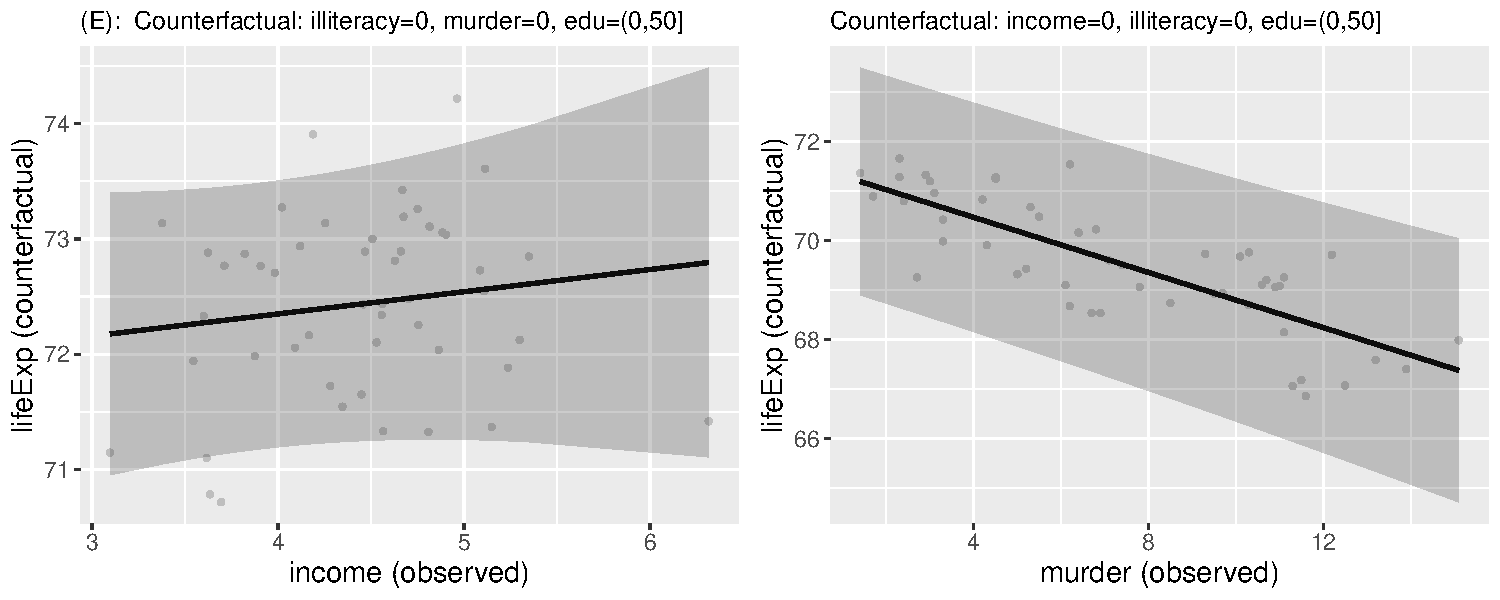
\includegraphics[trim={0 0 0 0},width=1\textwidth]{./figures/gg-lmpres-cifit.pdf}
\end{center}

In many case the uncertainty represented here is of little interest,
since it is the uncertainty of the intercept plus the exposure
effect. This is why even though the \texttt{murder} variable was highly
significant (p<0.001) whereas the income variable was not significant
(p=0.45) the confidence intervals looks large in both cases. To only
capture the uncertainty relative to the \texttt{income} or \texttt{murder} variable
one should remove the intercept value, e.g. by omitting
\texttt{"(Intercept)"} from the \texttt{var} argument:
\lstset{language=r,label= ,caption= ,captionpos=b,numbers=none}
\begin{lstlisting}
plot(e.lm, type = "partial", variable = "income", ci.alpha = 0.25) ## F
plot(e.lm, type = "partial", variable = "murder", ci.alpha = 0.25) ## G
\end{lstlisting}
\begin{center}
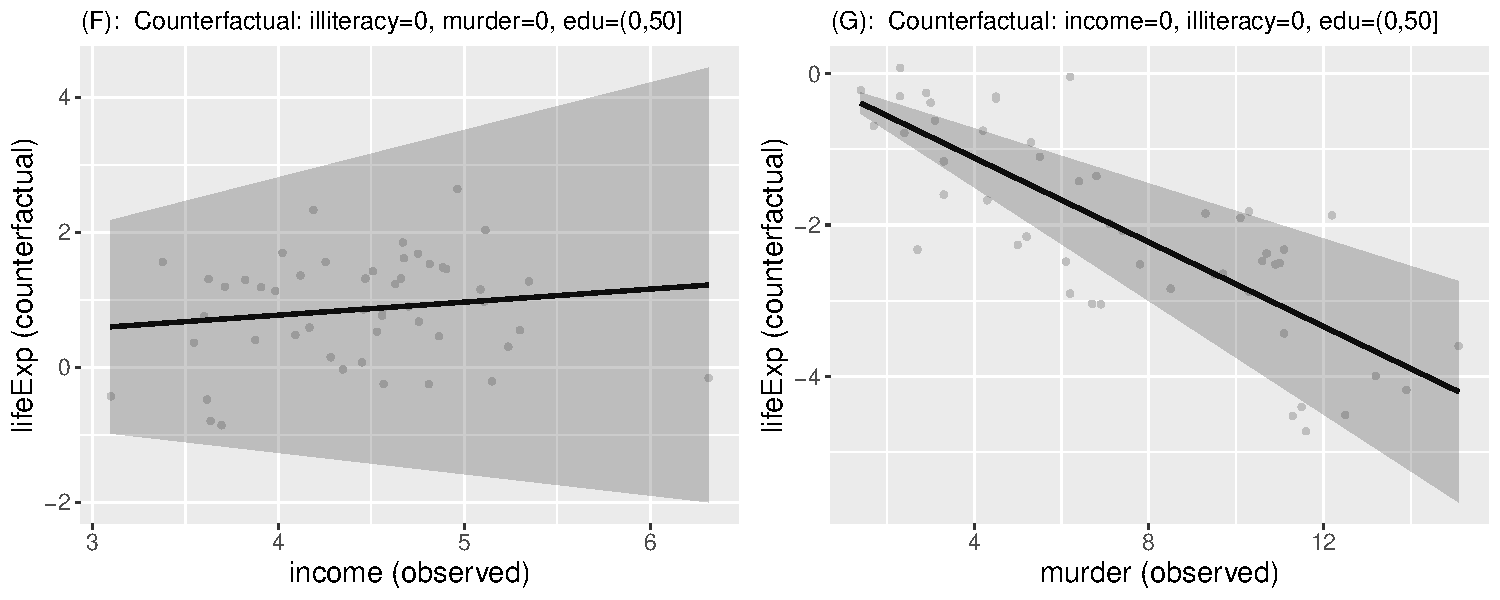
\includegraphics[trim={0 0 0 0},width=1\textwidth]{./figures/gg-lmpres-cicov.pdf}
\end{center}

The unpleasant side effect is that the range of values on the y-axis
appears unrealistic now. The statistical uncertainty may therefore be
better communicated otherwise, e.g. reporting confidence intervals or
p-values related to the covariate effect and keeping the partial
residual plot free of confidence intervals.

\subsection{Interaction with a categorical variable}
\label{sec:orgf90165c}

Suppose that we are now interested in relating life expectancy (\(Y\))
to both income (\(X_1\)) for various level of education (\(X_2 \in
\{a,b,c\}\)), adjusting for other variables such as illiteracy
(\(Z_1\)) and murder rate (\(Z_2\)). As before we assume a linear
effect for all variables:
\begin{align*}
Y = \alpha + \beta_{1a} X_1 \Ind[X_2=a] + \beta_{1b} X_1 \Ind[X_2=b] + \beta_{1c} X_1 \Ind[X_2=c] + \gamma_1 Z_1 + \gamma_2 Z_2 + \varepsilon
\end{align*}
where \(\Ind[x]\) denotes the indicator variable taking value 1 when
\(x\) is true and 0 otherwise. This model can be estimated with the
following R code
\lstset{language=r,label= ,caption= ,captionpos=b,numbers=none}
\begin{lstlisting}
e.lmI <- lmm(lifeExp ~ income:edu + illiteracy + murder, data = df1)
model.tables(e.lmI)
\end{lstlisting}

\begin{verbatim}
                   estimate       se     df    lower    upper    p.value
(Intercept)        71.78584 1.209517 44.009 69.34823 74.22344 0.0000e+00
illiteracy          0.12870 0.319145 44.009 -0.51449  0.77189 6.8871e-01
murder             -0.27940 0.048208 44.009 -0.37656 -0.18224 6.7276e-07
income:edu(0,50]    0.17147 0.297725 44.009 -0.42855  0.77149 5.6760e-01
income:edu(50,60]   0.22526 0.252110 44.009 -0.28284  0.73335 3.7646e-01
income:edu(60,100]  0.30377 0.236929 44.009 -0.17373  0.78126 2.0652e-01
\end{verbatim}


\uline{Note:} this model is the same as \texttt{lmm(lifeExp \textasciitilde{} income*edu +
illiteracy + murder, data = df1)} but uses a different parametrisation.

\bigskip

Similarly as before, we can use the \texttt{plot} function to display the
partial residuals with respect to both \texttt{income} and \texttt{edu}:
\lstset{language=r,label= ,caption= ,captionpos=b,numbers=none}
\begin{lstlisting}
plot(e.lmI, type = "partial", variable = c("(Intercept)","income","edu")) ## H
\end{lstlisting}

which can be compared to a plot assuming no interaction:
\lstset{language=r,label= ,caption= ,captionpos=b,numbers=none}
\begin{lstlisting}
plot(e.lm, type = "partial", variable = c("(Intercept)","income","edu")) ## I
\end{lstlisting}

\begin{center}
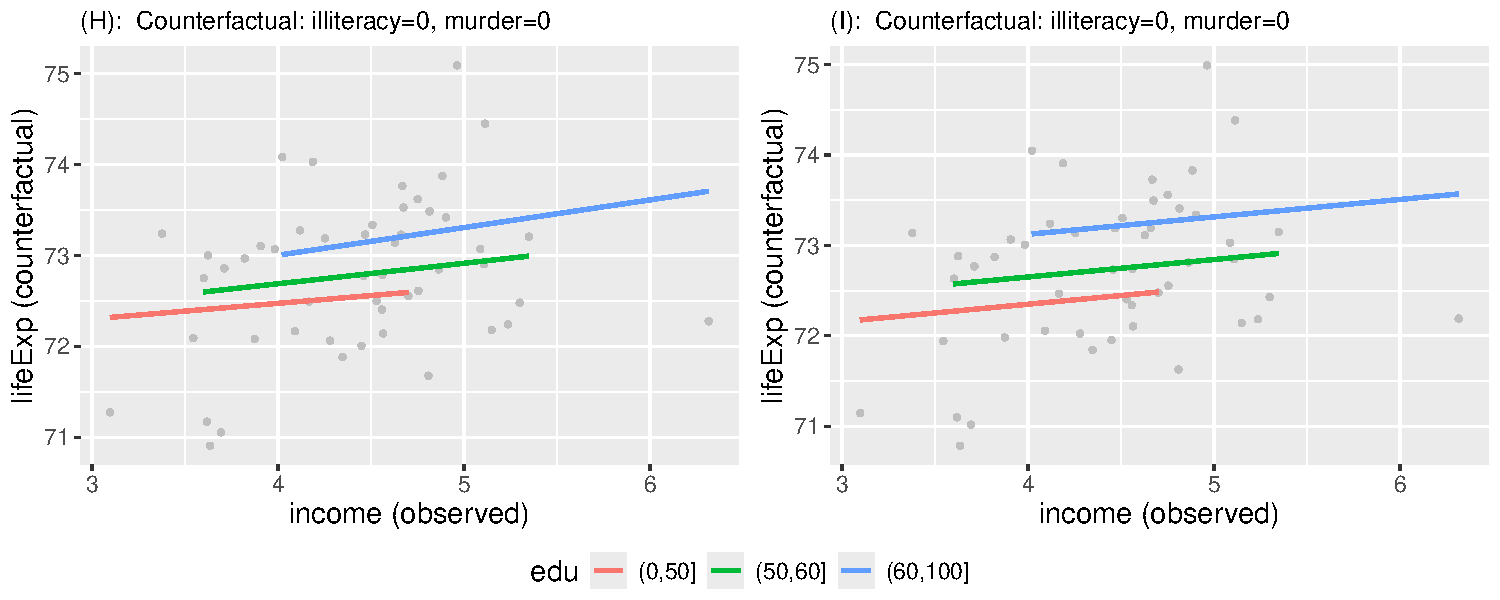
\includegraphics[trim={0 0 0 0},width=1\textwidth]{./figures/gg-lmpres-interaction.pdf}
\end{center}


The partial residuals can also be output via the \texttt{residuals} method:
\lstset{language=r,label= ,caption= ,captionpos=b,numbers=none}
\begin{lstlisting}
residuals(e.lmI, type = "partial", variable = c("(Intercept)","income","edu"))[1:5]
\end{lstlisting}

\begin{verbatim}
[1] 72.999 72.274 72.498 73.237 74.446
\end{verbatim}


and one can check that they are evaluated by substracting the effect
of the other variables (here \texttt{illiteracy} and \texttt{murder}), e.g.:
\lstset{language=r,label= ,caption= ,captionpos=b,numbers=none}
\begin{lstlisting}
c(69.05 - 0.12870 * 2.1 - (-0.27940) * 15.1,
  69.31 - 0.12870 * 1.5 - (-0.27940) * 11.3)
\end{lstlisting}

\begin{verbatim}
[1] 72.999 72.274
\end{verbatim}


Here we computed partial residuals representing the life expectancy in
the states had there be no murder nor illiteracy. We could also
consider the case of average murder rate and illiteracy:
\lstset{language=r,label= ,caption= ,captionpos=b,numbers=none}
\begin{lstlisting}
residuals(e.lmI, type = "partial", variable = c("(Intercept)","income"),
          at = data.frame(illiteracy = 1.17, murder = 7.378))[1:5]
\end{lstlisting}

\begin{verbatim}
[1] 71.088 70.363 70.587 71.327 72.535
\end{verbatim}


which we can also retrieve by hand:
\lstset{language=r,label= ,caption= ,captionpos=b,numbers=none}
\begin{lstlisting}
c(69.05 - 0.12870 * (2.1-1.170) - (-0.27940) * (15.1-7.378),
  69.31 - 0.12870 * (1.5-1.170) - (-0.27940) * (11.3-7.378))
\end{lstlisting}

\begin{verbatim}
[1] 71.088 70.363
\end{verbatim}



\clearpage

\section{Linear mixed model}
\label{sec:org4dfd538}

To illustrate the use of partial residuals we will use data from a
two-arm randomized trial comparing the quality of the vision over time
of patients under placebo vs. active drug. We first re-shape the data:
\lstset{language=r,label= ,caption= ,captionpos=b,numbers=none}
\begin{lstlisting}
data(armd.wide, package = "nlmeU")
armd.long <- reshape(armd.wide, direction ="long",
                     varying = paste0("visual",c(0,4,12,24,52)), times = c(0,4,12,24,52),
                     timevar = "week.num", v.names = "visual")
armd.long$week <- as.factor(armd.long$week.num)
\end{lstlisting}

and notice that the outcome (\texttt{visual}) and the covariate \texttt{lesion} can be missing:
\lstset{language=r,label= ,caption= ,captionpos=b,numbers=none}
\begin{lstlisting}
summarizeNA(armd.long)
\end{lstlisting}

\begin{verbatim}
frequency missing.pattern n.missing subject lesion line0 treat.f miss.pat week.num visual id week
     1106       000000000         0       0      0     0       0        0        0      0  0    0
       89       000000100         1       0      0     0       0        0        0      1  0    0
        1       010000000         1       0      1     0       0        0        0      0  0    0
        4       010000100         2       0      1     0       0        0        0      1  0    0
\end{verbatim}


This is why a warning is displayed when fitting the linear mixed
model:
\lstset{language=r,label= ,caption= ,captionpos=b,numbers=none}
\begin{lstlisting}
e.lmm <- lmm(visual ~ week*treat.f + lesion, data = armd.long, repetition =~week|subject)
\end{lstlisting}

\begin{verbatim}
Warning message:
In .lmmNormalizeData(as.data.frame(data)[unique(stats::na.omit(var.all))],  :
  Can only handle missing values in the outcome variable visual. 
  5 observations with missing values in "lesion" have been removed. 
  1 cluster has been removed.
\end{verbatim}


To visualize the model fit, we can display the fitted mean for each
level of baseline lesion:
\lstset{language=r,label= ,caption= ,captionpos=b,numbers=none}
\begin{lstlisting}
plot(e.lmm, facet = ~lesion, labeller = label_both, facet_ncol = 4)
\end{lstlisting}

\begin{center}
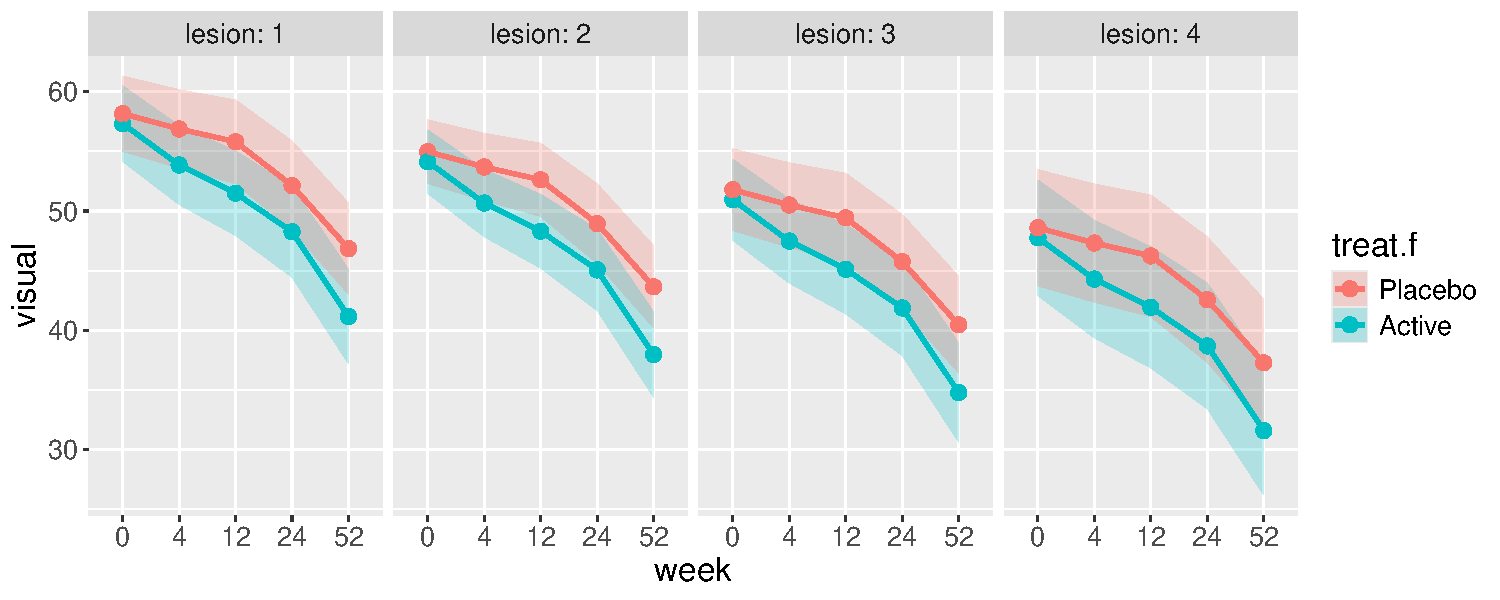
\includegraphics[trim={0 0 0 0},width=\textwidth]{./figures/gg-lmmfit.pdf}
\end{center}


We can retrive the fitted values from the estimated coefficients:
\lstset{language=r,label= ,caption= ,captionpos=b,numbers=none}
\begin{lstlisting}
round(coef(e.lmm),2)
\end{lstlisting}

\begin{verbatim}
         (Intercept)                week4               week12               week24 
               61.33                -1.28                -2.35                -6.03 
              week52        treat.fActive               lesion  week4:treat.fActive 
              -11.31                -0.84                -3.19                -2.19 
week12:treat.fActive week24:treat.fActive week52:treat.fActive 
               -3.47                -3.03                -4.84
\end{verbatim}


\begin{itemize}
\item in the Placebo group with lesion=1, the estimated average baseline mean
is \texttt{(Intercept)+1*lesion}, i.e. 61.33-3.19=58.14. When lesion=4, the
estimated average baseline mean is \texttt{(Intercept)+4*lesion},
i.e. 61.33-4*3.19=48.57.
\item the estimated average baseline mean in the Active group is shifted
by \texttt{treat.fActive} i.e. -0.84 from the Placebo group.
\item in the Placebo group with lesion=1, the estimated average week 52
mean is \newline \texttt{(Intercept)+week52+1*lesion},
i.e. 61.33-11.31-3.19=46.83.
\item the estimated average week 52 mean in the Active group is shifted by \newline
\texttt{treat.fActive+week52:treat.fActive} i.e. -0.84-4.84=-5.68 from the
Placebo group.
\end{itemize}

Unfortunately, the display of the fitted value becomes overwhelming
with considering more covariates or more covariate levels. Instead can
visualize the partial residuals, e.g. here the outcome and fitted
values had there be no lesion:
\begin{itemize}
\item on the same panel with a difference color for each treatment group:
\end{itemize}
\lstset{language=r,label= ,caption= ,captionpos=b,numbers=none}
\begin{lstlisting}
plot(e.lmm, type = "partial", variable = c("(Intercept)","week","treat.f"),
     at = data.frame(lesion = 2))
\end{lstlisting}

\begin{center}
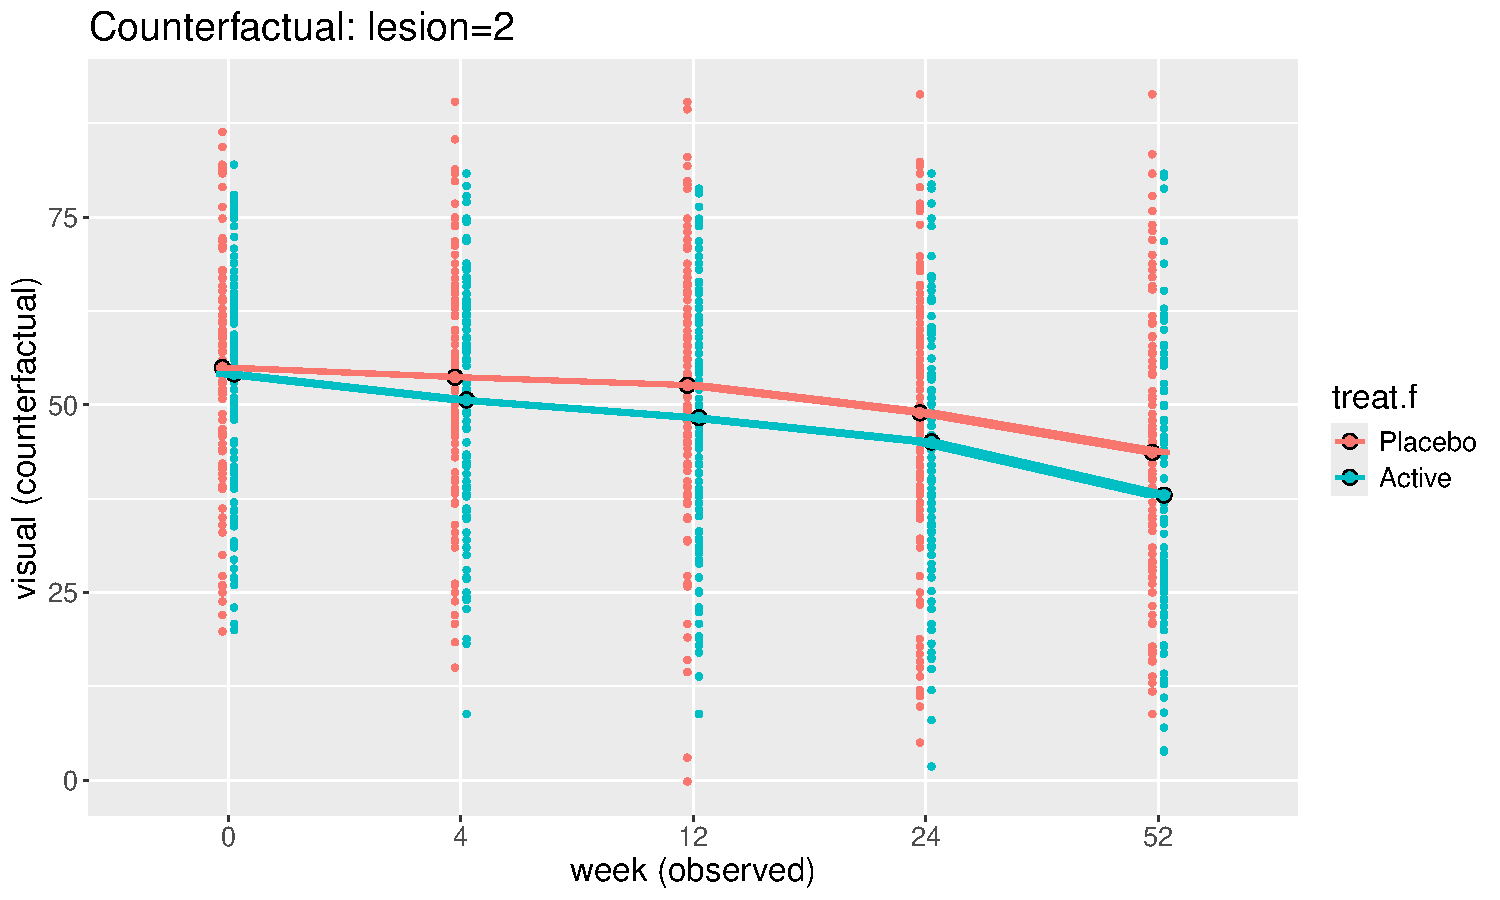
\includegraphics[trim={0 0 0 0},width=.8\textwidth]{./figures/gg-lmm-presTraj.pdf}
\end{center}



\begin{itemize}
\item on a separate panel for each timepoint:
\end{itemize}
\lstset{language=r,label= ,caption= ,captionpos=b,numbers=none}
\begin{lstlisting}
plot(e.lmm, type = "partial", variable = c("(Intercept)","week","treat.f"),
     facet =~week, facet_nrow = 1, time.var = "treat.f", color = FALSE,
     at = data.frame(lesion = 2))
\end{lstlisting}

\begin{center}
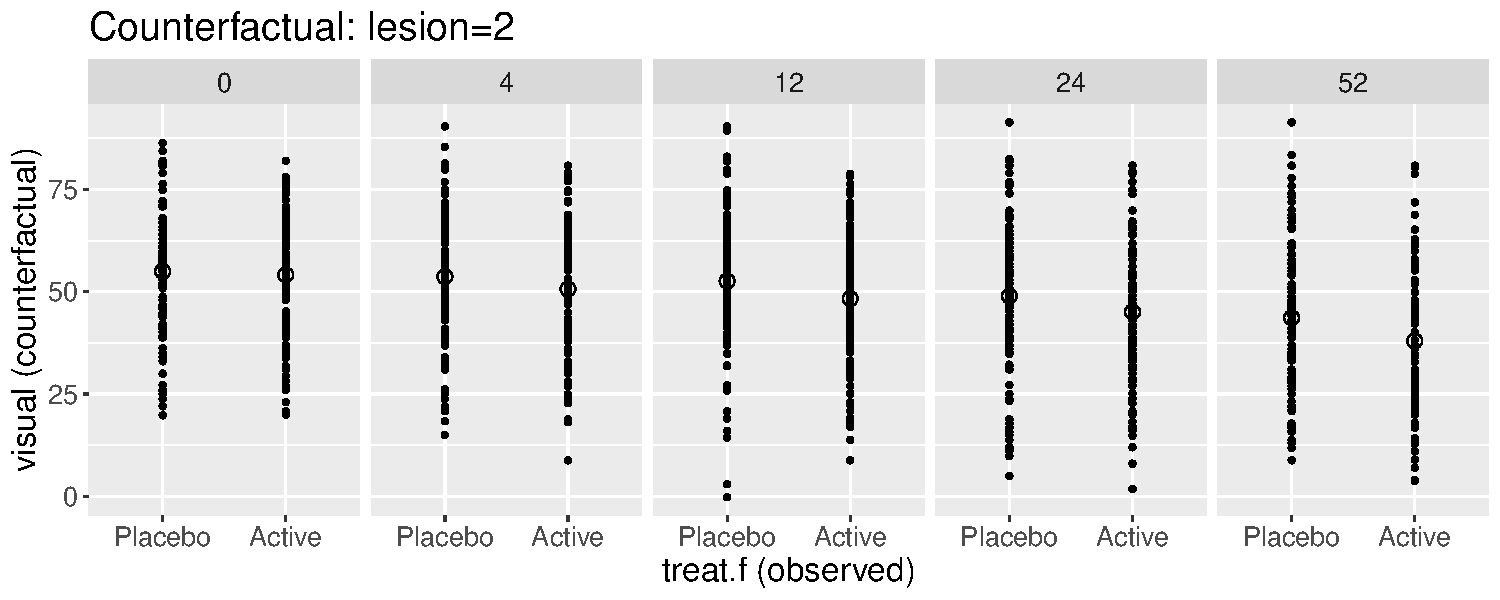
\includegraphics[trim={0 0 0 0},width=1\textwidth]{./figures/gg-lmm-presFacet.pdf}
\end{center}

The calculation of the partial residuals is similar to the univariate regression:
\lstset{language=r,label= ,caption= ,captionpos=b,numbers=none}
\begin{lstlisting}
armd.long$pres <- residuals(e.lmm, type = "partial", 
                            variable = c("(Intercept)","week","treat.f"),
                            at = data.frame(lesion = 2))
head(armd.long)
\end{lstlisting}

\begin{verbatim}
    subject lesion line0 treat.f miss.pat week.num visual id week   pres
1.0       1      3    12  Active     --XX        0     59  1    0 62.187
2.0       2      1    13  Active     ----        0     65  2    0 61.813
3.0       3      4     8 Placebo     ---X        0     40  3    0 46.373
4.0       4      2    13 Placebo     ----        0     67  4    0 67.000
5.0       5      1    14  Active     XXXX        0     70  5    0 66.813
6.0       6      3    12  Active     ----        0     59  6    0 62.187
\end{verbatim}


here substract the estimated lesion effect from the observed outcome:
\lstset{language=r,label= ,caption= ,captionpos=b,numbers=none}
\begin{lstlisting}
c(59 - (-3.19) * (3-2),
  65 - (-3.19) * (1-2))
\end{lstlisting}

\begin{verbatim}
[1] 62.19 61.81
\end{verbatim}


In particular, the partial residuals for patient with lesion equal to
two is the observed outcome.

\clearpage

\section{R session}
\label{sec:orged20498}
Details of the R session used to generate this document:
\lstset{language=r,label= ,caption= ,captionpos=b,numbers=none}
\begin{lstlisting}
sessionInfo()
\end{lstlisting}

\begin{verbatim}
R version 4.3.3 (2024-02-29)
Platform: x86_64-pc-linux-gnu (64-bit)
Running under: Ubuntu 22.04.4 LTS

Matrix products: default
BLAS:   /usr/lib/x86_64-linux-gnu/blas/libblas.so.3.10.0 
LAPACK: /usr/lib/x86_64-linux-gnu/lapack/liblapack.so.3.10.0

locale:
 [1] LC_CTYPE=en_US.UTF-8       LC_NUMERIC=C               LC_TIME=en_US.UTF-8       
 [4] LC_COLLATE=en_US.UTF-8     LC_MONETARY=en_US.UTF-8    LC_MESSAGES=en_US.UTF-8   
 [7] LC_PAPER=en_US.UTF-8       LC_NAME=C                  LC_ADDRESS=C              
[10] LC_TELEPHONE=C             LC_MEASUREMENT=en_US.UTF-8 LC_IDENTIFICATION=C       

time zone: Europe/Copenhagen
tzcode source: system (glibc)

attached base packages:
[1] stats     graphics  grDevices utils     datasets  methods   base     

other attached packages:
[1] lava_1.8.0    nlme_3.1-163  LMMstar_1.1.0 lme4_1.1-35.2 Matrix_1.6-5  ggpubr_0.6.0 
[7] ggplot2_3.5.1

loaded via a namespace (and not attached):
 [1] utf8_1.2.4          future_1.33.2       generics_0.1.3      tidyr_1.3.1        
 [5] rstatix_0.7.2       lattice_0.22-5      listenv_0.9.1       digest_0.6.35      
 [9] magrittr_2.0.3      grid_4.3.3          backports_1.4.1     survival_3.5-8     
[13] gridExtra_2.3       purrr_1.0.2         fansi_1.0.6         scales_1.3.0       
[17] numDeriv_2016.8-1.1 codetools_0.2-19    abind_1.4-5         cli_3.6.2          
[21] rlang_1.1.3         parallelly_1.37.1   future.apply_1.11.2 cowplot_1.1.3      
[25] munsell_0.5.1       splines_4.3.3       withr_3.0.0         tools_4.3.3        
[29] parallel_4.3.3      nloptr_2.0.3        ggsignif_0.6.4      minqa_1.2.6        
[33] dplyr_1.1.4         colorspace_2.1-0    boot_1.3-30         globals_0.16.3     
[37] broom_1.0.5         vctrs_0.6.5         R6_2.5.1            lifecycle_1.0.4    
[41] car_3.1-2           MASS_7.3-60.0.1     pkgconfig_2.0.3     pillar_1.9.0       
[45] gtable_0.3.5        glue_1.7.0          Rcpp_1.0.12         tibble_3.2.1       
[49] tidyselect_1.2.1    farver_2.1.1        labeling_0.4.3      carData_3.0-5      
[53] compiler_4.3.3
\end{verbatim}

\clearpage
\end{document}